\chapter{Results That Were Corrected}\label{app:superseded}

Three results of this thesis were first reported in a form that was later corrected. The
chapters give the corrected results. What was first reported is kept here, with what was wrong
with it, because the comparison between the two is part of the record
(\Cref{ch:reproducibility}) and a reader who meets an earlier version of this work should be
able to see what changed.

\section{The configuration as first reported}

The search over encoding, scheme, placement and batch was first reported as returning
$72.0$\,B per record against $174.3$\,B for the compression-only baseline, a reduction of
$58.7\%$ (\Cref{fig:e5}). That frame amortised one self-contained record over four frames and
so verified $0.881$ of its records at the loss rate it was specified for, not $0.95$. The
corrected figures are in \Cref{tab:ladder}.

\begin{figure}[h]
\centering
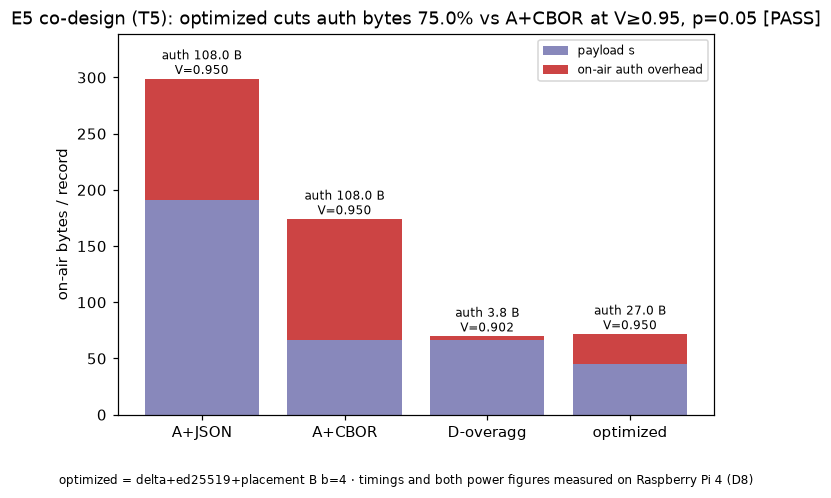
\includegraphics[width=0.7\textwidth]{fig_e5_codesign.png}
\caption[The configuration as first reported]{Per-record cost of the configuration as first
reported, against the two baselines (first format). Superseded by \Cref{tab:ladder}.}
\label{fig:e5}
\end{figure}

\section{The capacity envelope from one load ceiling}\label{sec:envelope-history}

Until October 2026 \Cref{ch:codesign} presented a ``capacity envelope'' computed, not simulated: the
$V \geq 0.95$ crossing had been measured once, at $N = 50$ with a $288$\,B frame, as a
utilisation $U = 2.435$ (offered load over saturation throughput), and that one ceiling was
applied to every configuration.

\begin{table}[h]
\centering
\caption{The envelope as previously reported, from the single load ceiling. \textbf{Superseded}
by \Cref{tab:ladder,tab:capacity}; kept because the comparison is the finding.}
\label{tab:envelope}
\begin{adjustbox}{max width=\textwidth}
\begin{tabular}{lrrrrrr}
\toprule
configuration & $\Lambda_i$ & $\Dmax$ & $b$ & $\Nmax$ ($U{<}1$) & $\Nmax$ ($V$ mean) & ($V$ per run) \\
\midrule
optimized delta/B & 50 & 100\,ms & 4 & 35 & 100 & 64--91 \\
A+CBOR (compression-only)  & 50 & 100\,ms & 1 & 18 & 31 & 24--29 \\
\midrule
optimized delta/B & 20 & 250\,ms & 4 & 103 & 213 & 163--201 \\
A+CBOR            & 20 & 250\,ms & 1 & 32  & 88  & 54--80 \\
\bottomrule
\end{tabular}
\end{adjustbox}
\end{table}

\begin{figure}[h]
\centering
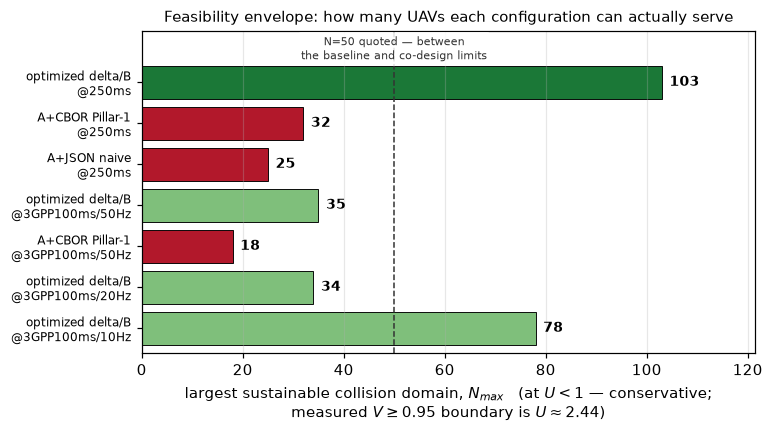
\includegraphics[width=0.75\textwidth]{fig_envelope.png}
\caption{The envelope as previously reported (saturation threshold). Superseded for the
$V \geq 0.95$ threshold by direct simulation.}
\label{fig:envelope}
\end{figure}

An earlier experiment had tested half of the assumption behind that ceiling --- that it does not
depend on frame size --- at $N = 50$ (\Cref{ch:validation}). The other half, that it does not
depend on $N$, was predicted to hold within $\pm 10\%$ in six configurations, and the prediction
was committed before the runs. \textbf{It failed.} The lean design crosses near $118$--$124$
nodes where the ceiling says $142$; the first format's shared-frame configuration crosses
\emph{above} the ceiling's value. The signs differ between configurations, so the ceiling cannot
be re-tuned. The reason is not subtle in hindsight: $U$ divides the offered load by the
saturation throughput of $N$ stations, which falls as $N$ grows, while the loss of a lightly
loaded network depends on how much airtime the traffic occupies and not on how many stations
produce it.

The ratios of the old envelope had been called ``protected by construction'', because numerator
and denominator used the same ceiling. They were protected against an error in the ceiling's
\emph{value}. They were not protected against the ceiling being the wrong \emph{kind} of
quantity, and they moved.

\section{Per-frame chaining as first computed}

On the low-rate arm, carrying the chain link once per frame was first reported to raise the
sustainable record rate by a factor of $3.0$ (\Cref{fig:lorachain}). The figure sized every
record from a delta measured with records $50$\,ms apart and carried no self-contained record.
At the spacing the batch itself implies, and with every frame decoding alone, the factor is
about $2.1$ in the first format (\Cref{sec:perframe}).

\begin{figure}[h]
\centering
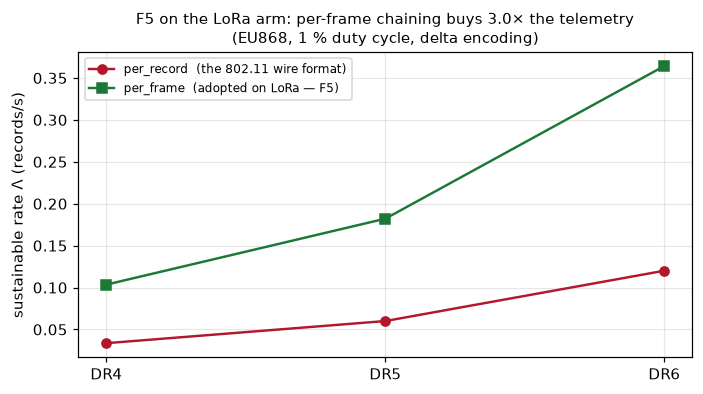
\includegraphics[width=0.7\textwidth]{fig_lora_chain.png}
\caption[Per-frame chaining as first computed]{Per-frame versus per-record chaining across data
rates, as first computed. Superseded by the table of \Cref{sec:perframe}.}
\label{fig:lorachain}
\end{figure}
